\chapter{Marco Teórico}

\section{Morfología}
La morfología humana estudia las estructuras del cuerpo humano desde distintos 
puntos de vista: se encarga de revisar los aspectos macroscópicos; 
también forma parte de la morfología humana el estudio microscópico
de los tejidos que lo conforman (histología) y también se incluye dentro del 
área de la morfología humana la forma en que se 
desarrollan los tejidos desde el momento de la concepción (desarrollo embrionario).

El estudio de la morfología humana sería entonces una integración de 
las disciplinas antes mencionadas. La anatomía es el área encargada de estudiar los 
aspectos macroscópicos de la estructura del cuerpo humano, como ya mencionamos,
la Histología se encarga de revisar los aspectos microscópicos de los tejidos 
y la disciplina llamada Ontogenia, es la que se dedica a estudiar el origen 
y desarrollo de los tejidos y las estructuras desde las etapas embrionarias.
En muchos cursos donde las distintas disciplinas de la biología  son una parte muy importante en la formación del alumno, las áreas que abarca la morfología 
humana se estudian por separado. En muchos cursos de medicina aparecen la Histología, Embriología y la Anatomía Humana como materias separadas.\\
El concepto antiguo sobre Morfología humana se refería simplemente al estudio de las formas y  las estructuras del organismo humano. 
El concepto moderno de la Morfología humana comprende no sólo el estudio de las estructuras, sino también el modo en que éstas se desarrollan, 
la manera en que funcionan y cómo se relacionan con el medio.\\
Con el avance de los conocimientos científicos, las áreas abarcadas por la morfología se han ido expandiendo, y han surgido nuevas áreas relacionadas con la morfología, 
como por ejemplo la Anatomía patológica (que estudia cortes de tejidos, para determinar  si son normales o presentan algún tipo de alteración).\\
Dentro de los métodos de investigación utilizados para estudiar la morfología humana, tenemos la disección de cadáveres, practicada desde los inicios de la Medicina, 
para conocer las estructuras del cuerpo humano. También se han practicado técnicas que incluyen la inyección de sustancias coloreadas en los vasos, conductos u órganos huecos. 
Otra técnica que ha permitido el avance en los conocimientos de la morfología humana es la inyección de líquidos solidificables, que al cambiar de estado proporcionan información 
sobre la forma del vaso u órgano hueco dentro del cual fue inyectado. Los rayos X y todas las técnicas imagenológicas desarrolladas en los últimos tiempos 
(tomografía axial computarizada, resonancia magnética, etc.) también han aportando importantes conocimientos en ésta área.\\
Desde el punto de vista microscópico, el desarrollo de distintas tecnologías (microscopía electrónica, de fluorescencia) ha colaborado también con la profundización de los 
conocimientos del área de la morfología humana.\\

\section{Sistemas del cuerpo Humano}
El cuerpo humano es una estructura compleja y altamente organizada, formada por células que trabajan juntas para realizar funciones específicas necesarias 
para mantener la vida.\cite{web17} La biología del cuerpo humano incluye:
\begin{itemize}
	\item Fisiología (cómo funciona el cuerpo).
	\item Anatomía (cómo se estructura el cuerpo).	
\end{itemize}
Para efectos de este trabajo terminal y los alcances del mismo solamente se trabajará con la anatomia humana.\\
La anatomía está organizada por niveles, desde los componentes más pequeños de las células hasta los órganos más grandes, así como su relación con otros órganos.\\
La anatomía general estudia los órganos tal como aparecen a simple vista o en una disección del cuerpo.\\
La anatomía celular es el estudio de las células y sus componentes, los cuales pueden observarse solo con la ayuda de técnicas e instrumentos especiales como los microscopios.\\
La anatomía molecular (a menudo llamada biología molecular) estudia los componentes más pequeños de las células al nivel bioquímico.\\
\begin{figure}[H]
\begin{center}
	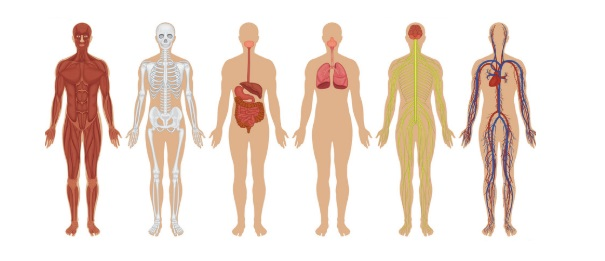
\includegraphics[width = .7\textwidth]{source/images/image22.png}
 	\captionof{figure}{\label{fig:im23}Los sistemas del cuerpo humano.\cite{web11}}
	\end{center} 
\end{figure}

\section{Sistema Digestivo}
La cavidad abdominal 
es el espacio corporal que ocupa la región del abdomen, ubicada entre el diafragma y la abertura de la pelvis. 
Es la cavidad más grande del cuerpo humano 
a diferencia de las demás cavidades,ver \ref{fig:im24}, y 
contiene los principales órganos del aparato digestivo, urinario y genital.
Para su estudio y evaluación clínica en el campo de la medicina, 
el abdomen debe ser dividido topográficamente de forma externa en 9 
cuadrantes o regiones, utilizando cuatro líneas 
trazadas imaginariamente, dos verticales y dos horizontales, ver \ref{fig:im24}.\cite{web12}
\begin{figure}
 \begin{center}
  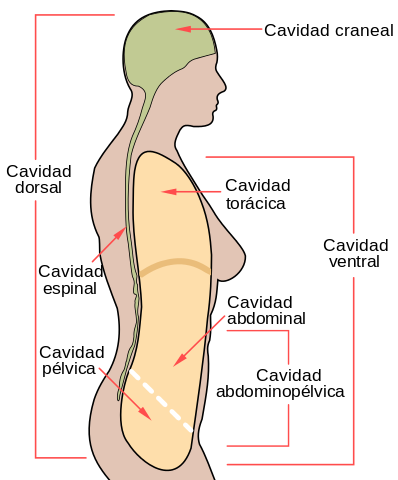
\includegraphics[width = .3\textwidth]{source/images/image56.png}
  \captionof{figure}{\label{fig:im24}Cavidades del cuerpo humano.}
 \end{center} 
\end{figure}

\begin{figure}[H]
	\begin{center}
 		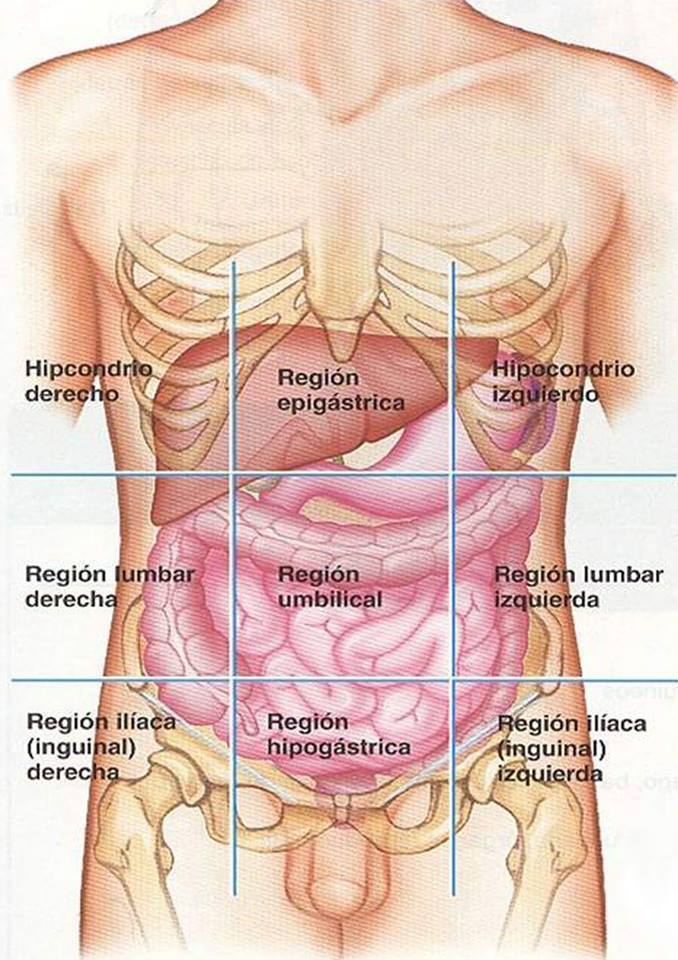
\includegraphics[width = .3\textwidth]{v3/images/image1.jpg}
 		\captionof{figure}{\label{fig:im24.0}Cuadrantes de la cavidad abdominal.}
	\end{center} 
\end{figure}
A continuación se presenta un resumen de los conceptos basicos de los elementos que conforman la cavidad abdominal\cite{pró2012anatomía}:
\begin{itemize}
	\item El \textbf{abdomen} es la región que se encuentra entre el tórax y la pelvis. El diafragma separa las estructuras del tórax de las del abdomen. 
	\item La \textbf{abertura} superior de la pelvis comunica la pelvis con la cavidad abdominal.
	\item La \textbf{pared abdominal} se encuentra compuesta por piel, tejido subcutáneo, planos musculares con sus aponeurosis y fascias y peritoneo parietal.
	\item La \textbf{cavidad abdominal} se encuentra integrada por la cavidad peritoneal, el retroperitoneo y las vísceras peritonizadas.
	\item La \textbf{cavidad peritoneal} se encuentra limitada por las láminas visceral y parietal del peritoneo.
	\item El \textbf{retroperitoneo} está integrado por todas las estructuras anatómicas que se encuentran por detrás de la lámina parietal posterior del peritoneo.
	\item La \textbf{cavidad abdominal} incluye estructuras pertenecientes a los sistemas digestivo, endocrino, vascular, nervioso y urinario.
	\item Las \textbf{vísceras sólidas} de la cavidad abdominal son el hígado, el bazo, el páncreas, los riñones y las glándulas suprarrenales.
	\item Las \textbf{huecas} son el tubo digestivo y las vías de excreción urinaria. 
	\item El \textbf{tubo digestivo abdominal} está integrado por el esófago (porción abdominal), el estómago, el duodeno, el yeyuno, el íleon y las porciones del colon (ciego, apéndice vermiforme, colon ascendente, transverso, descendente y sigmoide).
	\item El \textbf{sistema vascular} incluye las arterias ramas de la porción abdominal de la aorta, las venas tributarias de la cava inferior y la vena porta hepática y los linfáticos.
	\item La \textbf{porción abdominal de la arteria aorta} se extiende desde el hiato aórtico del diafragma y sus ramas terminales son las arterias ilíacas comunes. Se encuentra en situación prevertebral desplazada hacia la izquierda de la columna lumbar. 
	\item La \textbf{vena cava inferior} se forma por la anastomosis de ambas ilíacas comunes y asciende en situación prevertebral desplazada a la derecha hasta el orificio de la vena cava en el diafragma.
	\item La \textbf{vena porta hepática} se forma detrás de la cabeza del páncreas por la anastomosis de las venas esplénica (que ya recibe como afluente a la vena mesentérica inferior) y mesentérica superior, y se dirige al hígado dentro del omento menor.
	\item Los \textbf{troncos linfáticos} de los miembros inferiores, la pelvis y el abdomen confluyen detrás de la cabeza del páncreas donde se origina el conducto torácico. Este asciende y atraviesa el diafragma por el hiato aórtico en dirección al tórax.
\end{itemize}
A continuación se muestra una imagen,ver \ref{fig:im25}, del sistema digestivo (El epiplón mayor
\footnote{ también llamado omento o reaño, es un pliegue bilaminar del peritoneo situado en el abdomen. Se extiende desde el estómago y la porción proximal de duodeno hasta órganos adyacentes de la cavidad abdominal.} 
ha sido parcialmente eliminado o reflejado)  está contienen la información de cuáles son los órganos y elementos que lo conforman, estos serán 
varios ya que se han tomado como guía, estos elegidos mediante a una entrevista de estudiantes de medicina como material que se ha utilizado para el estudio del cuerpo 
humano, para la realización de modelos en 3D del presente trabajo. ejemplifica el material que dispone pero no limitado a el alumnado para el estudio del sistema en cuestión.\\
\begin{figure}[H]
	\begin{center}
 		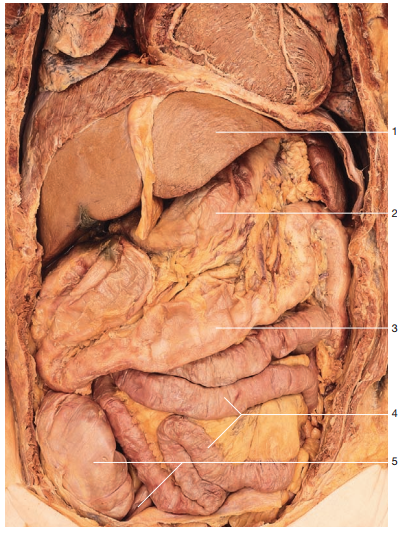
\includegraphics[width = .5\textwidth]{source/images/image72.png}
 		\captionof{figure}{\label{fig:im25}Órganos digestivos in situ\cite{rohen2018anatomy}}
	\end{center} 
\end{figure}
\begin{enumerate}
	\item Hígado
	\item Estómago
	\item Colon transverso
	\item Intestino delgado
	\item Ciego con apéndice vermiforme	
\end{enumerate}
En el apendice se puede encontrar la información detallada de los componentes y organos del sistema digestivo.

\section{Realidad Virtual}
Algunos autores definen así la Realidad Virtual.\\
\newline
\textit{“La realidad virtual (RV) es una simulación tridimensional generada o asistida comúnmente por computadora de algún aspecto del mundo real o ficticio, en el cual 
el usuario tiene la sensación de pertenecer a ese ambiente sintético o interactuar con él”}\cite{web6}\\ 
\textbf{Corrado Padila Érica}\\
\newline
“Realidad Virtual: gráficos 3D en entornos inmersivos que usan I/O
artefactos como guantes, cascos, etc. en busca de mayores grados de iteración
con el ambiente virtual”\cite{web7}\\ 
\textbf{Lozano Miguel, Calderón}\\
\newline
"Realidad Virtual es una forma en que los seres humanos puedan
visualizar, manipular e interactuar con las computadoras y datos extremadamente
complejos".\cite{web8}\\
\textbf{Isdale, Jerry}\\
\newline
“Un sistema interactivo capaz de crear una simulación que implique a varios de los sentidos del ser humano, generados por una computadora, explorable, visualizable y manipulable 
en tiempo real; este bajo la forma de imágenes y sonidos, estos, dando la sensación de presencia en el entorno generado”\cite{web9}\\
\textbf{Levis, Diego}\\
\newline
Esta última ha sido la definición que se ha tomado para el desarrollo del proyecto del trabajo terminal, asimismo se puede concluir que todos los autores coinciden en que la 
realidad virtual es un mundo simulado en el que el usuario puede interactuar en tiempo real por medio
de dispositivos o computadoras que logran un efecto artificial e inmersivo en el que se pueden manipular objetos.

\section{La Realidad Virtual en la Educaci\'on}
Los estudiantes deben aprender que se pueden conquistar nuevas fronteras cruzando los límites disciplinarios. En el caso de la tecnología y el proceso educativo, 
se deben crear oportunidades de aprendizaje que atraviesen la psicología, la sociología, la historia, la filosofía, la antropología, la ciencia y la teoría organizacional, 
construyéndose hacia sistemas complejos de comprensión aplicables a problemas complejos. Esto es tan cierto para comprender a los alumnos individuales como para comprender 
la cultura colectiva.\\
A pesar del potencial de la interacion de tecnologias de la información, en este caso la RV, pueden derivarse de un enfoque integrado y transdisciplinario, 
todavía es necesario ubicar el pro dentro de las estructuras administrativas y los contenidos academicos de la Universidad.\\ 
La inclusión de este topo de tecnologías refleja una imagen de indagación que trasciende y se centra en cuatro amplios dominios de indagación.\cite{norton1994integrating}
\begin{enumerate}
	\item \textbf{Impactos de la tecnología en los contextos sociales}a través de exploraciones de la historia de la tecnología, el papel de la tecnología en el cambio, los impactos sociales, globales, económicos, políticos y psicológicos de la tecnología, la integración de la tecnología a medida que impacta en diversas culturas y las implicaciones de los cambios actuales para el diseño de práctica educativa.
	\item \textbf{Impactos de la tecnología en las formas de conocimiento} a través del examen de las influencias psicológicas y epistemológicas de la tecnología sobre la naturaleza del conocimiento - sobre lo que sabemos y cómo lo conocemos - al indagar sobre la estructura y las implicaciones de las diversas arenas de discurso social y estructural creadas por las tecnologías electrónicas.
	\item \textbf{Impactos de la tecnología en el proceso de aprendizaje} a través de investigaciones de definiciones emergentes de entornos de aprendizaje consistentes con configuraciones sociales más amplias y con visiones más nuevas del proceso de aprendizaje, pensamiento, resolución de problemas y creativo, incluida la naturaleza y el papel de las estrategias de instrucción y concepciones más amplias de los atributos y características del alumno.
	\item \textbf{La tecnología impacta en los objetivos educativos a través de la reevaluación de los objetivos educativos tradicionales}, repensando lo que se debe aprender, cómo se debe aprender, quién es el alumno, la naturaleza de las experiencias culturales de cada alumno y cómo se puede evaluar el aprendizaje, en particular el la naturaleza transdisciplinaria del conocimiento y el aprendizaje y la literatura emergente sobre estándares y metas para la educación, así como el papel de la tecnología en la configuración de estas reevaluaciones.
\end{enumerate}
Todo esto \dots %Pendiente...
\subsection{Participación Programable}
Las características de la realidad virtual son las mismas que las de una buena enseñanza. El profesor quiere crear un entorno que sea programable y en el que 
participen los alumnos. "El principio más importante del diseño de actividades en el aula es que las acciones del estudiante determinan lo que se aprenderá". 
Es decir, la atención es lo primero, el aprendizaje después de la atención está enfocada. Y el aprendizaje es principalmente acción.\\ 
La idea es simple, todo lo que hacemos para educar con palabras y con imágenes se puede brindar como experiencia virtual. Podemos variar ubicación, escala, densidad de información, 
interactividad y capacidad de respuesta, tiempo, grado de participación.\\
La idea es simple, todo lo que hacemos para educar con palabras y con imágenes se puede brindar como experiencia virtual. Podemos variar ubicación, escala, densidad de información, 
interactividad y capacidad de respuesta, tiempo, grado de participación.
\subsection{Semántica Natural}
La interacción de la RV está acoplada al comportamiento natural. La regla general es que un niño debe poder controlar el sistema. Sin líneas de comando o clics del mouse, 
más bien, simplemente caminar y señalar y hablar y agarrar.\\
La realidad virtual tiene sentido cuando lo que un participante ve y oye tiene un significado que no requiere explicación. Piense en una casa. 
Una descripción textual requiere habilidades de lectura, una base de datos de procedimientos (listas de coordenadas) requiere decodificación, una imagen puede reconocerse 
inmediatamente pero no es interactiva. Una casa en realidad virtual se parece más a una casa física, puedes mirarla mientras caminas alrededor, puedes caminar por la puerta 
principal y explorar cada habitación. Una casa física tiene semántica natural, nadie necesita explicarla. La semántica natural es lo que aprende un niño antes de la escolarización 
simbólica.
\subsection{Constructivismo}
Los entornos virtuales no se limitan solo a la visualización, el alumno puede interactuar con objetos y espacios en la realidad virtual. El alumno puede utilizar herramientas para crear 
nuevos entornos, modificar los antiguos, realizar exámenes de simulación, corregir errores, jugar, en lugar de enseñar una estructura de símbolos y luego enseñar el significado de esa 
estructura, en RV. Primero enseñaremos el significado a través de la experiencia, luego (si es necesario) enseñaremos la abstracción simbólica de nuestras experiencias.\\
Pero la computadora es una herramienta ideal para manipular las abstracciones simbólicas. En lugar de enseñar la abstracción, podemos simplemente enseñar cómo usar la herramienta 
de realidad virtual, una interfaz natural con abstracciones. La RV no es una simulación de la realidad, es un superconjunto de la realidad.\\
La realidad virtual enseña la construcción activa del medio ambiente. Los datos no son una lista abstracta de números, los datos son lo que percibimos en nuestro entorno. 
El aprendizaje no es una lista abstracta de palabras de libros de texto, es lo que hacemos en nuestro entorno. El plan de estudios oculto de la realidad virtual es: haz tu mundo y 
cuídalo. Prueba los experimentos de forma segura. Experimente las consecuencias, luego elija del conocimiento lo que sea necesario.
\subsection{Presencia Cognitiva}
En la realidad virtual, cada objeto se puede habitar como un cuerpo virtual. Los estudiantes no son simplemente coparticipantes, trayendo su perspectiva dentro del mismo contexto de un objeto, 
sino que los estudiantes pueden convertirse en el objeto, ver y actuar en el mundo virtual como si fuera el objeto. \cite{bricken1990learning}

\section{Modelado 3D}
En general, independientemente de la disciplina, el proceso de modelado es una simplificación de un objeto para su posterior estudio o representación. 
Así, podemos hablar de modelos matemáticos que simplifican fenómenos físicos, o modelos meteorológicos para la predicción del tiempo atmosférico, etc.
 Un modelo geométrico define la información sobre la forma (geometría) de un determinado objeto. Las simplificaciones que se realicen en su definición 
 vendrán determinadas por diferentes factores como el método de representación utilizado, operadores empleados o nivel de detalle.\cite{web13} \\
Se puede definir el proceso de modelado geométrico tridimensional como el encargado de crear modelos consistentes que puedan ser manejados algorítmicamente 
en un computador. Este proceso de construcción se aborda en diferentes etapas, partiendo típicamente de entidades básicas y aplicando una serie de operadores 
sobre ellas. Estas entidades básicas pueden ser primitivas geométricas (calculadas de forma algorítmica o mediante una ecuación matemática) u obtenidas mediante 
un dispositivo de captura (escáner 3D).\\
Existen multitud de técnicas de modelado 3D. En una primera taxonomía de alto nivel podemos hacer una categorización dependiendo de si el modelado se centra 
en definir únicamente las características del contorno del objeto, los siguiente son los mas usados:\\
\begin{itemize}
\item \textbf{Modelado Sólido:} también conocidos como de Geometría Sólida Constructiva (CSG Constructed Solid Geometry). Los modelos sólidos definen el volumen 
del objeto que representan, y en muchos casos indican incluso el centro de masas, la densidad del material interna, etc. Se utilizan en fabricación por computadora 
y en aplicaciones médicas e industriales.
\item \textbf{Modelado de Contorno:} también conocidos como de Representación de Contorno (B-Rep - Boundary Representation). Los modelos de contorno únicamente 
representan la superficie límite del objeto (de forma conceptual, la "cáscara"). Son más fáciles de definir y modificar. Además, lo interesante para la representación 
del objeto es su apariencia exterior (en los casos donde interesa el interior simplemente se aproxima, como en el caso del SubSurfaceScattering). Prácticamente todos 
los paquetes de diseño y animación (incluido Blender) empleados en síntesis de imagen y en aplicaciones interactivas emplean este tipo de modelos.
\end{itemize}
Para  cubrir las necesidades de los modelos 3D de los órganos del sistema digestivo se ha opto por que estos fueran realizados en el modelado de contorno por su facilidad 
de desarrollo y ligereza de carga en el renderizado en el momento de la implementación de estos en el sistema de realidad virtual.\\

\section{Generacion de Entorno 3D}
El entorno 3D es en donde el usuario se encontrará al ingresar al sistema de realidad virtual, para, este se ha realizado para dar la sensación de encontrarse en un ambiente médico.\\
Se utilizaron modelos ya realizados por un autor adquiriendo los derechos de uso ya que la realización de estos no se consideran parte integral del desarrollo del Trabajo Terminal, 
escrito esto no se quiere demeritar la necesidad de hacer el usuario ya que, como se ha mencionado en secciones anteriores, se tiene énfasis en la experiencia del usuario para que 
la inmersión del usuario sea la mayor posible.\\
\begin{figure}[H]
	\begin{center}
 		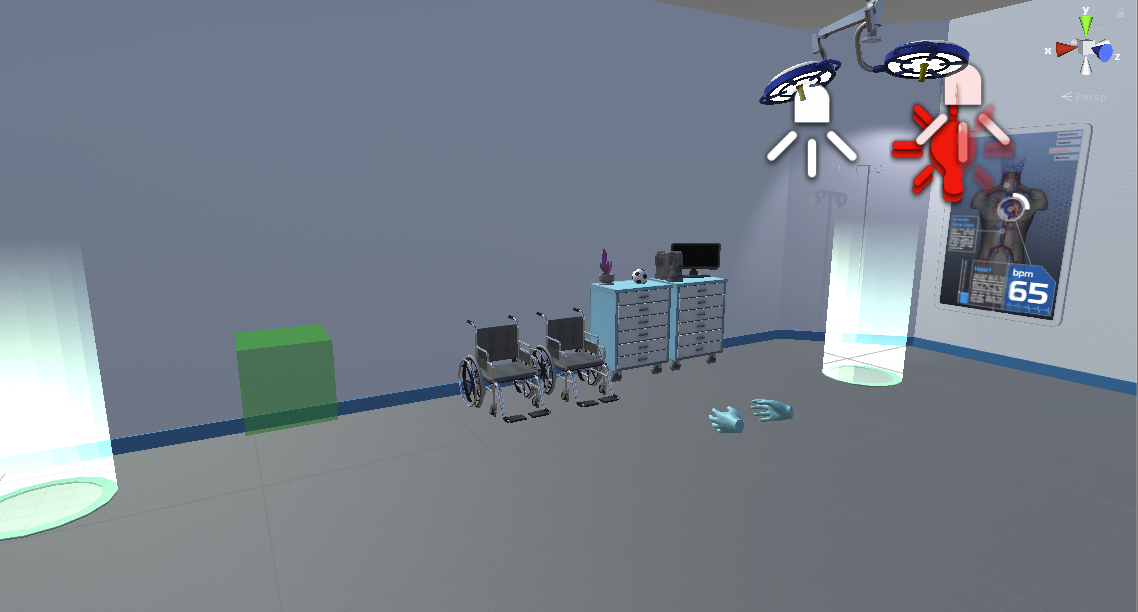
\includegraphics[width = .5\textwidth]{source/images/image63.png}
 		\captionof{figure}{\label{fig:im31}Entorno 3D vista normal}
	\end{center} 
\end{figure}

\begin{figure}[H]
	\begin{center}
 		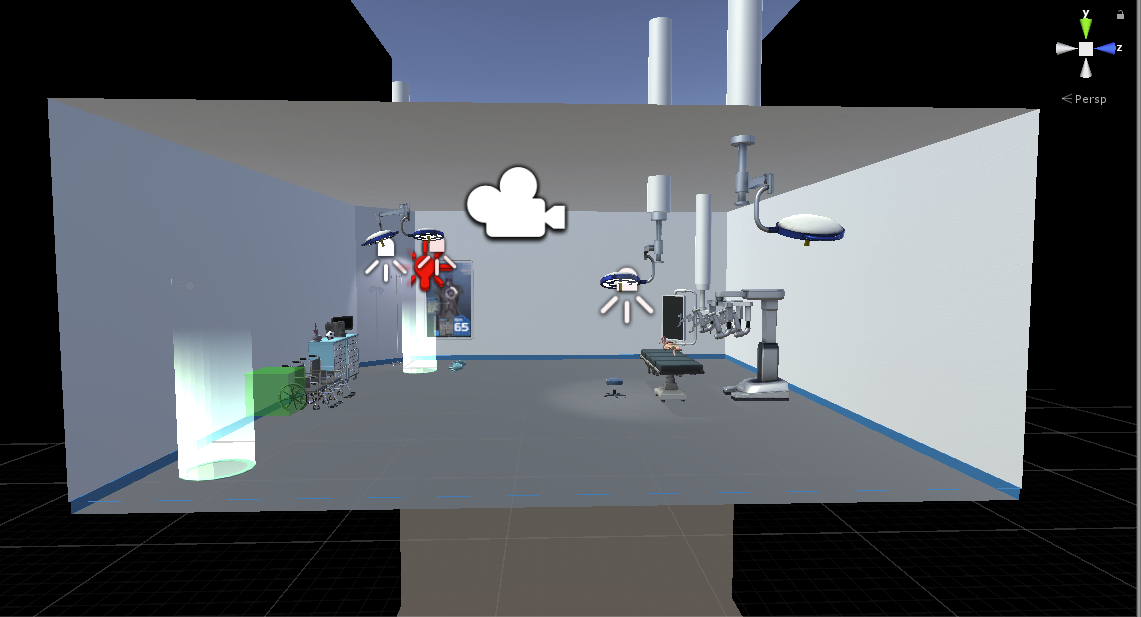
\includegraphics[width = .5\textwidth]{source/images/image53.png}
 		\captionof{figure}{\label{fig:im32} Entorno 3D vista externa de la escena}
	\end{center} 
\end{figure}

\begin{figure}[H]
	\begin{center}
 		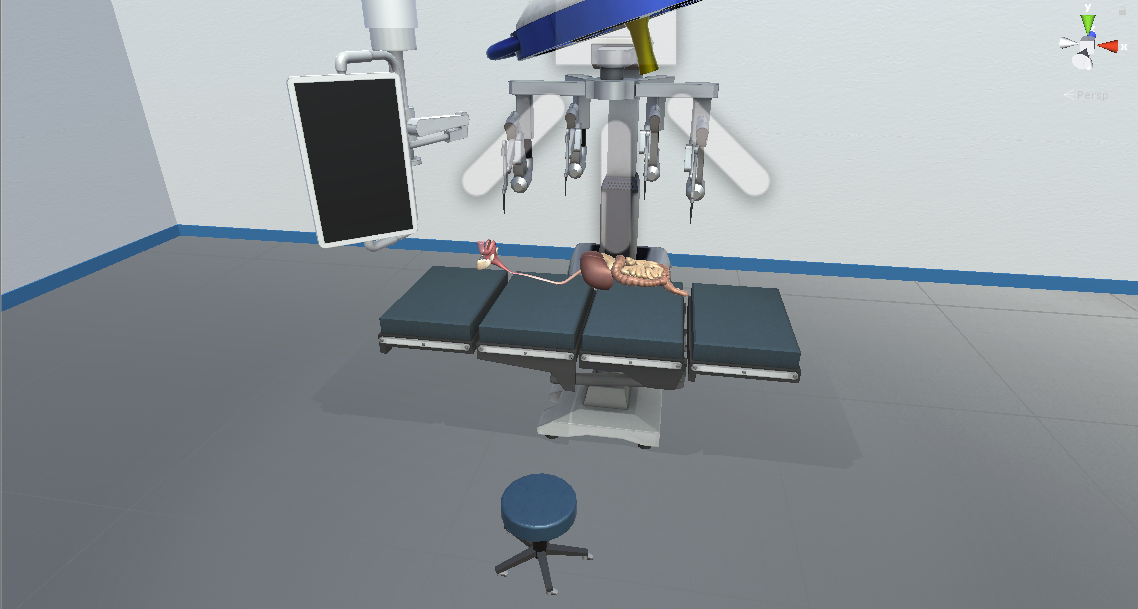
\includegraphics[width = .5\textwidth]{source/images/image16.png}
 		\captionof{figure}{\label{fig:im33}Entorno 3D  vista principal}
	\end{center} 
\end{figure}


% (Aquí puede decir lo de unity y demás cosas que se requieren para hacer lo que usted ya hizo)
%(Tratemos de usar lo que se tiene y solo añadir si es indispensable, recortar si es necesario para añadir a Apendices, como lo de las imagenes del aparato digestivo que estaban en el primer documento)
